%%%%%%%%%%%%%%%%%%%%%%%%%%%%%%%%%%%%%%%%%%%%%%%%%%%%%%%%%%%%%%%%%%%%
%% I, the copyright holder of this work, release this work into the
%% public domain. This applies worldwide. In some countries this may
%% not be legally possible; if so: I grant anyone the right to use
%% this work for any purpose, without any conditions, unless such
%% conditions are required by law.
%%%%%%%%%%%%%%%%%%%%%%%%%%%%%%%%%%%%%%%%%%%%%%%%%%%%%%%%%%%%%%%%%%%%

\documentclass[
  digital, %% This option enables the default options for the
           %% digital version of a document. Replace with `printed`
           %% to enable the default options for the printed version
           %% of a document.
  table,   %% Causes the coloring of tables. Replace with `notable`
           %% to restore plain tables.
  nolof,     %% Prints the List of Figures. Replace with `nolof` to
           %% hide the List of Figures.
  nolot,     %% Prints the List of Tables. Replace with `nolot` to
           %% hide the List of Tables.
  nocover,
  color
  %% More options are listed in the user guide at
  %% <http://mirrors.ctan.org/macros/latex/contrib/fithesis/guide/mu/fi.pdf>.
]{fithesis3}
%% The following section sets up the locales used in the thesis.
\usepackage[resetfonts]{cmap} %% We need to load the T2A font encoding
\usepackage[T1,T2A]{fontenc}  %% to use the Cyrillic fonts with Russian texts.
\usepackage[
  main=english, %% By using `czech` or `slovak` as the main locale
                %% instead of `english`, you can typeset the thesis
                %% in either Czech or Slovak, respectively.
  english, german, russian, czech, slovak %% The additional keys allow
]{babel}        %% foreign texts to be typeset as follows:
%%
%%   \begin{otherlanguage}{german}  ... \end{otherlanguage}
%%   \begin{otherlanguage}{russian} ... \end{otherlanguage}
%%   \begin{otherlanguage}{czech}   ... \end{otherlanguage}
%%   \begin{otherlanguage}{slovak}  ... \end{otherlanguage}
%%
%% For non-Latin scripts, it may be necessary to load additional
%% fonts:
\usepackage{paratype}
\def\textrussian#1{{\usefont{T2A}{PTSerif-TLF}{m}{rm}#1}}
%%
%% The following section sets up the metadata of the thesis.
\thesissetup{
    date          = \the\year/\the\month/\the\day,
    university    = mu,
    faculty       = fi,
    type          = bc,
    author        = Dominik Gmiterko,
    gender        = m,
    advisor       = Radek Pelánek,
    title         = {Techniques for measuring similarity of educational items},
    TeXtitle      = {Techniques for measuring similarity of educational items},
    keywords      = {similarity, measure, keyword2, ...},
    TeXkeywords   = {similarity, measure, keyword2, \ldots},
    abstract      = {This is the abstract of my thesis, which can

                     span multiple paragraphs.},
    thanks        = {These are the acknowledgements for my thesis, which can

                     span multiple paragraphs.},
    bib           = thesis.bib,
}
\usepackage{makeidx}      %% The `makeidx` package contains
\makeindex                %% helper commands for index typesetting.
%% These additional packages are used within the document:
\usepackage{paralist} %% Compact list environments
\usepackage{amsmath}  %% Mathematics
\usepackage{amsthm}
\usepackage{amsfonts}
\usepackage{hyperref} %% Hyperlinks
\usepackage{markdown} %% Lightweight markup
\usepackage{listings} %% Source code highlighting
\hypersetup{colorlinks, urlcolor=[rgb]{0.6,0.2,1.0}, linkcolor=[rgb]{0.0,0.0,0.0}}
\lstset{
  basicstyle      = \ttfamily,%
  identifierstyle = \color{black},%
  keywordstyle    = \color{blue},%
  keywordstyle    = {[2]\color{cyan}},%
  keywordstyle    = {[3]\color{olive}},%
  stringstyle     = \color{teal},%
  commentstyle    = \itshape\color{magenta}}
\usepackage{floatrow} %% Putting captions above tables
\floatsetup[table]{capposition=top}
\begin{document}

\newcommand{\ppl}[1]{\textcolor[rgb]{0.6,0.2,1.0}{#1}}
\newcommand{\umimeCesky}{\ppl{Umíme česky}}
% \newcommand{\umimeCesky}{Umíme česky}

\hyphenpenalty=9999
\exhyphenpenalty=10000

\hypersetup{linkcolor=[rgb]{0.6,0.2,1.0}}

\chapter*{Introduction}
\addcontentsline{toc}{chapter}{Introduction}

% --------------------------- %
% Introduction                %
% --------------------------- %

% interactive educational systems
% focus on systems with a large number of items

Tutoring systems are computer-based systems designed to introduce users into various domains. They usually hold a large number of items which enables them to provide a personalized experience. To maintain this large pool of items efficiently we need to be able to decide which items are useful and which are not.

% one possible method, using similarity of items

One possible way how to achieve this is to use similarity of items. Similarity is basic metric which can be then used in various use-cases, e.g., projections, clustering, outlier detection. Work discusses different possible similarity measures and differences between them.

% our similarity

% goal of this work

Main part of this work consists exploitative analysis of one such tutoring system. We were trying to find different aspects in tutoring system which can affect similarity measure and explain them. This work focuses on tutoring systems with thousands of items as such similarity measure is most useful for them. In particular we used data from tutoring system \umimeCesky{}.

% structure of this work

Besides Introduction and Conclusion chapters, this thesis is structured into three additional chapters. First chapter talks in general about the problem of measuring the similarity of educational items and advantages of using similarity. This chapter also describes previous work and different proposed measures for computing similarity. Later we explain different types of data available in tutoring systems. The second chapter then advances level deeper and describes observed problems specific to data we are using.
The last chapter gives an overview of many experiments that were concluded and summarizes results.

This is draft from \today %TODO remove!

\chapter{Similarity}

% --------------------------- %
% Similarity                  %
% --------------------------- %

% Intro to chapter, structure

In this chapter, we talk in general about items (questions) in tutoring systems and computing their similarity. At the beginning of the chapter, we focus on better explaining basic terms like tutoring system, item, and similarity which will be used all through the work. We also describe different kinds of data available about items and possible measures for calculating similarity.
The last section of this chapter describes data used in our experiments. In particular, we describe used dataset and outline ways of simulating artificial data.

% > Tutoring systems

\section{Tutoring systems}\label{tutoring-systems}

Tutoring systems are computer systems which purpose is to teach its users (students) some knowledge or skill. These systems do this autonomously to some degree. The degree of automation may vary for each tutoring system.

% Autonomous aspects of tutoring systems

Many different aspects of learning may be implemented into the system or they may also be left out. The most common task which tutoring systems solve is choosing a most beneficial item from the pool of items available for users to solve. This can be done in some simple way or system may also adapt to each of the users choosing more challenging and interesting items to users who are more skilled in a specific area. While presenting users who struggle with more basic items. This is beneficial for maximizing learning aspect of the system. [CITE?] Another aspect which can tutoring systems solve is providing hints and feedback to students. When there are teachers interacting with the system we can also provide feedback about their students progress and so on.

% Recommender systems

One closely related area are recommender systems which differ from tutoring systems only slightly. Both areas are observing users and items. The main difference is that our main source of information is a performance of users while solving specific item and recommender systems mostly use rating of the items. Which in fact are still only numbers representing slightly different things so we can still share some of the techniques. Although different goals bring different problems specific to each area.

% Main difference from educational systems

One difference is that we can use some additional data about items. There are item statements and solutions of students which can in some contexts give us really useful information about items.

% > Items

\section{Items}\label{items}

% Why this term

In this work, we use the term ``items'' which may refer to problems, questions, assignments in different systems. Item is a single entry in an educational system which
users can answer to. Since many aspects of this work are generally applicable we decided to use this broad term. Complexity of single item in tutoring system can differ greatly. In some tutoring systems, this may refer to simple choice from two options while in other one item is complex
tasks which user solves in a matter of minutes.

% Data sources

To further specify the context of our research, we will describe characteristics of items. Computing similarity may be performed by different measures, but they all have to use data which are available for each item. Therefore we first describe sources of data that can be utilized for measuring the similarity of items.

\begin{itemize}
\item
  \textbf{Item statement} is some specification of the item for a learner to solve, e.g., a natural language description of the task. Another commonly used format is a grid. Many systems focusing on logic puzzles and programming problems use it.
\item
  \textbf{Item solutions} may provide us with additional information about an item. There will usually be some sample solution provided by the author and we can also utilize all the solutions from users.
\item
  \textbf{User's performance} consists of information provided indirectly by users. Performance of items may represent user solving times, correctness of the answers, number of attempts required.
\end{itemize}

Structure of both item statement and solutions differ greatly based context of tutoring system. However, in general, it is still possible to convert data into some standard form and use one of a few standard measures despite original representation.

This description of an item is broad enough to cover most of the tutoring systems. End of this chapter discusses more closely tutoring system used for our results.

%%% Tutoring systems contain educational items; the large pool is required in some contexts

The most important property of tutoring systems is that they contain educational items which are solved by users. However, amount of items in systems may vary. Some tutoring systems require a large number of items. This is especially true when they practice simple facts instead of skills. In personalized tutoring systems, the need for a large pool of items is even higher. When providing personalized questions we need a wider set of items to choose from.

%%% It may be useful to determine the similarity of items

Dealing with a large pool of items may not be easy. To maintain a pool of items efficiently we need to be able to easily decide which items are useful and which are not. One possible tool which can help us here is similarity of items.

% > Measuring similarity

\section{Measuring similarity}\label{measuring-similarity}

The following section is explaining general approach to measuring and using similarity of educational items.

% what is a similarity, how can we compute it

In general, we can compute the similarity of items in many ways. We define measures for computing similarity for two items. Then when we want to use similarity for some specific use-case we compute pairwise similarities for all pair of items.

Items in our context are commonly represented as vectors of numeric values. For performance data, this is a vector of correctness or time from all users to given item. Other properties of items like question statement may also be represented as a vector, e.g., by using bag-of-words.

When we have vectors for each item we can compare them pairwise to get similarity using some standard similarity measures like Pearson correlation coefficient, cosine similarity, Sokal measure or Euclidean distance.

% Edit distance

Another possible way to measuring similarity is counting edits which would convert one item to another. This is called edit distance and there are standard ways of computing it for both strings and trees. Edit distance can be then converted into similarity using something like $1 / (1 + \text{edit distance})$. Therefore this covers another common group of information we can encounter.

% > > Standard pipeline

\subsection{Standard pipeline}\label{standard-pipeline}

To we can wrap it up. There are a few data structures and few calculations involved in the standard pipeline for computing similarity of educational items.

\begin{enumerate}
  \item
    \textbf{Feature matrix} is matrix (items $\times$ features) containing source data. As we said previously this can represent any property of the items. This matrix consists of one vector for each item and it may represent item statement, solution or solutions of the item and naturally even users performance.
  \item
    \textbf{Measuring similarity} may involve some similarity measure or edit distance. This step is used to compute the similarity between all pairs of items. In other words, we transform feature matrix into similarity matrix.
  \item
    \textbf{Similarity matrix} is matrix (item $\times$ item) where each value represents similarity of pair of items.
  \item
    \textbf{Dimensionality reduction} is used to transform similarity matrix into a projection. Techniques like PCA or t-SNE may be used for this.
  \item
    \textbf{Projection} is more compact representation (item $\times$ 2) of similarity matrix used for visualizations for end users. There are other possible use-cases of similarity like clustering, outlier detection but we are focusing on projections.
\end{enumerate}

% > Why is similarity of items useful

\section{Why is similarity of items useful}\label{why-is-similarity-of-items-useful}

% Managing problem pool

As we mentioned previously key part of learning is solving educational items. Defining some measures for computing similarity of items can then be used for different purposes.

First, most direct, usage is a recommendation of items for a student to solve. We do not want to recommend very similar items to those that were solved without any problems. However when user struggled system should consider recommending more of the similar problems to strengthen users knowledge.

Another possible usage is generating hints by selecting examples which are similar to the item which is currently solved. Examples are selected from a database of examples. This usage of similarity was used by [CITE Hosseini; Brusilovsky].

Two previous use cases were using problem similarity to automatically make some choices inside tutoring system. Another approach is to bring humans into the decision-making loop [CITE]. This approach provides authors of tutoring system with visualizations which should inform them what changes may be useful. E.g. detecting redundant problems and pointing out where there are not enough similar problems.

One possible way of achieving this is plotting problems to plane and displaying it to the author. This still can not be used for a very large amount of items. But we choose this approach for our specific data as they contain a large number of items but can be divided into item-sets which are solved independently in the system.

One of the use cases of visualizations is a detection of outliers - items which behave differently than others. This behavior is directly shown in projection and such items lie far away from others.

There is one more usage of similarity which we won't be discussing further. The similarity of items can be utilized for automatic construction of clustering and hierarchical categorization. Even when author already has items categorized he can compare it to computed categorization to verify that groups are formed correctly and refine them if needed.

%TODO mention visualizations, clustering and outlier detection explicitly

\chapter{Used data and techniques}\label{used-data-and-techniques}

% --------------------------- %
% Used datasets               %
% --------------------------- %

The first half of this chapter focuses on used sources of data. It describes both simulated data and dataset from the actual system.
We outline structure of tutoring system and focus on exercises and its objects that are useful for our work. Another section includes basic statistics about data from \umimeCesky{}. We also summarise previous work using the same dataset.

After that second half of the chapter gives a detailed description of pipeline used in our experiments when calculating similarity and projections. End of the chapter,contains example of the simple projection and description of what properties should it have to be useful.

% types of data (real, simulated), why, real, simulated

In our analysis, we use both real data from the educational system and simulated data. Reason for this is that real-world data are useful for concluding any practical results. However, evaluation of this data is often complicated as we do not know the truth about many of its aspects. That is why we also use simulated data for validating some of our conclusions.

% > Simulated data

\section{Simulated data}\label{simulated-data}

So when simulating data we are trying to generate results which are similar to real tutoring system. However, we use much simpler model.

The result of the simulation consists mainly of performance matrix with items as columns and users as its rows. First, we have to generate items. For each item, we choose its difficulty and skill required to solve this item. The difficulty of item is value drawn from normal distribution $\mathcal{N}(0,\,1)$.

After that, we continued with the construction of users. We generate skills for all users - a matrix of $u$ users and all used skills. This matrix is also filled with random values from normal distribution $\mathcal{N}(0,\,1)$.

Next, we simulate each user answering to each item. User answers correctly whenever is a random value higher than a logistic function of the difference of item difficulty and user skill. When it is not given answer is incorrect. User skill is one of the skills which corresponds to the skill required for given item.

We will talk more in depth about how we generated simulated data in next chapter when describing how we used them specifically. In all experiments using simulated data, we altered this basic simulation in some way to achieve results corresponding to some attribute of real data.

% > Umime cesky

\section{\umimeCesky{}}\label{umime-cesky}

% Czech grammar, ``fill-in-the-blank'' with two choices

\href{https://umimecesky.cz/}{Umíme česky} is a system for practice of Czech grammar. The system contains multiple exercise types, but in our analysis, we use only one exercise type - simple ``fill-in-the-blank'' with two possible answers. A user is asked to choose one of them.

\begin{figure}
  
\includegraphics[width=7cm]{img/umimecesky_doplnovacka}
  \caption{Sample question from ``fill-in-the-blank'' exercise in \umimeCesky{}}
  \label{fig:umimeceskydoplnovacka}
\end{figure}

Although we focused only on ``fill-in-the-blank'' exercise it can still be used to train various concepts of Czech grammar. The exercise contains many questions and they are divided into item-sets. Each item-set consists of items practicing a different aspect of language, e.g., ``Vyjmenovaná slova po B'' or ``Velká písmena: státy, oblasti''. This item-sets are arranged into hierarchical categorization as seen in the user interface. As our analysis works only with item-sets separately this categorization into different aspects is important to our work. We consider results from each item-set as it has uniform items, but we do not compare them against each other.

Items in item-sets are then divided into levels. Where higher levels are intended for solving by more experienced users as they contain more difficult questions. In general, there are three difficulty levels but not all item-sets have all three of them. Some easy item-sets include only first level. On another hand, there are item-sets which have all three levels or only higher levels.

% information about items: question, correctness and time

The used dataset contains multiple sources of information about items. In ``item statement'' group it is a statement of the question with one missing spot and two possible answers to fill in there. We also know answers from all the users. Then in performance group of information, it is correctness of user answers and response time.

It is not possible to use response time directly. We need to normalize it in some clever way as raw response time is greatly affected by both lengths of questions and users reading speed. Also, it is a good idea to use logarithm of time instead of time itself. This is shown by [CITE]. Only then it would be useful to use data about response times. This is a reason why we are using mostly correctness of user answers.

% Why this system

We choose this tutoring system because, as we explained before, we are focusing on problems which are most important for systems with a large number of items. Also provided dataset has a large number of users and answers which is great for the stability of results.

% > > Basic statistics

\subsection{Basic statistics}\label{basic-statistics}

\begin{table}
  \begin{tabular}{|l|r r r r|}
    \hline
     & Items & Users & Answers & Item-user answers \\
    \hline\hline
    Whole exercise & 6\,037 & 46\,128 & 10\,421\,521 & 7\,264\,763 \\
    \hline
    One item-set & 273 & 14\,207 & 1\,216\,403 & 888\,748 \\
    \hline
  \end{tabular}
  \caption{Basic statistics of dataset}
  \label{tab:basic-statistics}
\end{table}

This section provides some basic statistics about the size of dataset and users of the system. Table \ref{tab:basic-statistics} shows number of items, users and answers. Statistics are both global and for one selected item-set which is the one most commonly used for analysis. This item-set has most answers from users, therefore, it is ideal for analysis as results are more stable. We used this item-set by default but we also confirmed observed behavior on other item-sets. The last column (``Item-user answers'') contains a count of unique item-user pair which were answered. This number differs from all logged answers because users can answer the same item multiple times. In this case, we use only one of the answers for further analysis.

% Users using the system

A primary group of users using \umimeCesky{} are children studying at primary and secondary school. Users can have individual accounts
but the system also allows teachers to create a virtual class and assign students to it. A teacher is then able to select some exercises and give them to students to solve until some deadline. Each week about 200 classes visit the system.

% > Previous work

\section{Previous work}\label{previous-work}

Dataset from \umimeCesky{} was used previously in few articles and thesis. Most of the work relevant to our problem comes from article Measuring Similarity of Educational Items Using Data on Learners’ Performance [CITE].

They compared few chosen similarity measures to each other. The result was that some of the similarity measures correlate greatly and some do not. It was also determined which similarity measures it is best to use for the stability of results. Especially that using Pearson correlation coefficient is a good default choice.

We are also using it for several reasons. The described article showed that it has good enough results in producing distinct clusters on performance data. Another reason is that Pearson correlation is easy to use as many computational environments already contain fast implementation.

The article also showed that using ``second level of similarity'' improves the stability of results further. However, we choose not to use it as our dataset is large enough to be sable even with a simpler measure. Using straightforward measure is also beneficial when explaining results and this factor is important to our work.

% Description of common projection output

\section{Used techniques}\label{Used techniques}

% why is projection useful

Projections come in handy when it is hard to understand data directly because there is way too much of them. And this is our case as we focus on systems which consist of thousands of solvable items and even more users. Projections are results of dimensionality reduction techniques. We project many-dimensional data into 2 thoughtfully chosen dimensions to simplify them.

% similarity and projection

In general, we want projection which puts similar items together. This can be achieved in many different ways. The following section explains choices we made when selecting a source of data, a method of processing them prior to applying dimensionality reduction, and dimensionality reduction technique itself.

% > > Computation of item similarity

\subsection{Computation of item similarity}\label{computation-of-item-similarity}

% How is a projection (similarity) computed

To better understand how were projections created we have to understand steps of their computation. We call this process a default pipeline and it is used in most cases. When some of the further analysis modify it slightly it is pointed out in the corresponding section. Whenever we don't specify so all projections were produced using this default pipeline.

% Performance matrix

The first step we have to take is converting raw logged information about user answers into \textbf{performance matrix}. Columns of the matrix are items in the educational system and each row of the matrix contains data about single user's performance. In our case, we used correctness of first users answer to specific item as his performance. This means value 1.0 in case of the correct answer and 0.0 for incorrect. It is worth mentioning that performance matrix is relatively sparse as it is not common for users to solve all the items in the system.

% Similarity matrix

Next step is computing \textbf{similarity matrix}. It is filled with a pairwise correlation of all items from the performance matrix. For this was chosen Pearson correlation coefficient based on previous work. Values produced by correlation are between $-1$ and $+1$. Each value in this matrix represents similarity of two items. This gives matrix some properties - matrix is symmetric and all values at main diagonal are 1.0.

% PCA, (TSNE)

The last step is producing 2D \textbf{projection}. The similarity matrix is useful for a computer to directly make a decision based on it. However, this matrix still contains way too many values for a human to interpret. As some of our goals are explaining data to authors of the system. We continue with a dimensional reduction to produce a more compact representation of data. This can be achieved by using any dimensional reduction technique.

% PCA over TSNE

We decided to use Principal component analysis (PCA) and first two principal components are then used for 2D visualizations. We choose PCA over other commonly used technique t-SNE (which can produce better-looking results) for one important reason. Results of PCA are deterministic. It produces the same result for same input each time it is run. This is not true for t-SNE which is technique using machine learning and gradient descent for finding some local extreme. Stable results are more suitable for understanding data as there is no variation to results caused by the algorithm. And it is much easier to compare results when altering measure used for computing item similarities.

% Why this pipeline, performance data (not item statement)

We choose this specific pipeline as we think it is utilizing data about items which hold most information about their similarity. Other possible choices are using item statement and solutions provided by students. However, they do not hold as much information in our specific tutoring system. Item statements in our observed exercise consist only of few Czech words with one missing spot. And student solution is basically only selection from two provided options. Item statement and solutions can be used more effectively in other contexts like programming, mathematics, or physics where item statements are much more complex.

Also performance is easier to transfer into different tutoring systems because performance is usually available and contrary to item statement performance can be expressed using standard format - performance matrix.

This choice of a pipeline is also relatively easy to understand. As it consists only of few steps which can be studied separately and interchanged.

\section{Visible properties of projections}\label{visible-properties-of-projections}

% Visible Properties of projection

\begin{figure}
    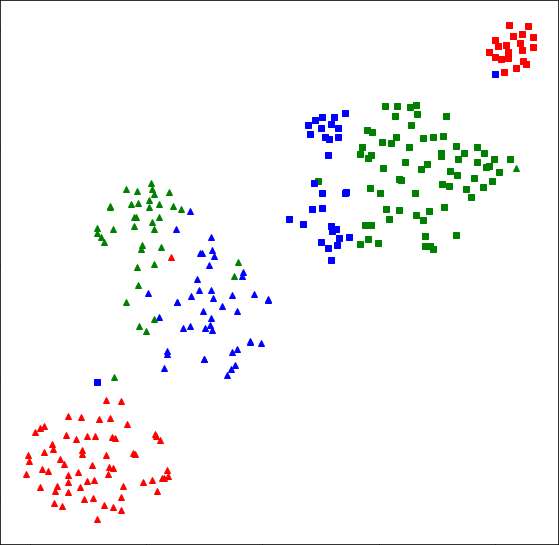
\includegraphics[height=8cm]{img/common_projection}
  \caption{Basic t-SNE projection of one item-set (``Vyjmenovaná slova po B'')}
  \label{fig:common_projection}
\end{figure}

Figure \ref{fig:common_projection} shows how can resulting projection look like. This particular projection shows 273 items (single item-set). Each item is represented as one dot in the image and its proximity to others represents how similar they are.

% Similar words near each other

As projections are meant to be used for managing item pool this puts some constraints on how ideal projection should look like.

We want similar items to end as close to each other as possible. When we use performance as data source we can also interpret as items which require same skills are projected near each other - their answers from each user correlate. For example, when we look at our selected item-set we can see that all words starting with ``bio'' are close to each other. This group consists of words which are indeed similar because they are based on a single word with added suffix. But remember, there is no information about item statement presented to the similarity measure.

% > Regularities

\section{Regularities}\label{regularities}

% This causes similar words to end-up far away one from another

Projections of item-sets from system \umimeCesky{} (look back at Figure \ref{fig:common_projection}) all display some regularities. Items depicted with same colors and items using same markers form clusters. But so far we have not explained what properties of items colors and used markers represent. This section talks about formed clusters in projection and why it may be a problem.

% > > Level regularity

\subsection{Level regularity}\label{regularities-level-regularity}

% Description of problem, 3 clusters based on 3 levels of questions difficulty

Figure \ref{fig:common_projection} contains items of three different colors. Item-sets in system \umimeCesky{} are divided into multiple levels of difficulty. For this particular item-set, there are three difficulty levels. The first level is depicted using red (with 110 items), second green (with 86 items), and third blue (with 77 items). There is a  visible pattern in our data - each cluster consists mostly of items item from one level.

As we mentioned before, only data about user performance (correctness of answers) are used when composing projections. And there is not a direct reason for this clusters of same levels to form as no information about belonging to a particular level is presented to the algorithm.

% why is this unsuitable, example of similar words far away one from another

This phenomenon is not suitable for analysis of item similarity as it can cause misleading results about similarity. One particular example is when similar words are displayed far away from one another just because they belong to different levels. Such example is pair of words ``bič'' and ``bičík'' in item-set ``Vyjmenovaná slova po B''.

% > > Answers regularity

\subsection{Answers regularity}\label{answers-regularity}

Another property of items in figure \ref{fig:common_projection} is depicted by a marker used. One type of marker (rectangle) shows items with correct answer ``i'' and another marker (triangle) shows items with correct answer ``y''. Again, there is no direct information about this presented to measure of similarity but such clusters form despite it.

In our particular context of Czech language items should be similar only when they have same correct answer. So this regularity should not cause any problems with projection directly but it is still useful to explore why is this behavior present at all.

% general to be continued text

General question we are trying to address is why does calculation of similarity in this way project to clusters of levels and correct answers. Whole following chapter is focusing on this question.

% --------------------------- %
% Evaluation                  %
% --------------------------- %

\chapter{Evaluation}\label{evaluation}

The chapter is explaining factors that can affect resulting projections produced from real-world data. We are focusing on higher level factors that can cause a formation of clusters in projection. On a low level, it is apparent that items which performance correlates will be similar (close to each other) in projection. But we focus on higher-level factors in tutoring systems that can cause this correlation.

\section{Basic}\label{evaluation-basic}

The first section is focusing on experiments which determine a range of this behavior - whether distinct clusters of different answers and levels are still present when altering parameters of pipeline used to calculate projection.

\subsection{First and last users answer}\label{first-and-last-users-answer}

% Why bother about this

Our performance matrix contains only one value for each item-user pair. But users can possibly answer to the item multiple times. This raises a question about which of user answers to use. [CITE]

% What we used in performance matrix

We tried using both first users answer and last in performance matrix. However, there is no visible difference in results. This is clear when we compare first and last answers of users. There is only 5\% different answers between them. So at least with a large number of items in the system it does not really matter which one is chosen as only a few items are answered multiple times.

\subsection{Quality of clusters on different item-sets}\label{quality-of-clusters}

When introducing the problem of unneeded clusters in section \ref{regularities} we showed that one particular item-set shows this behavior. However, we still do not know whether this is true for all the item-sets. We decided it may be useful to quantify how recognizable are this clusters on all item-sets.

% Quantification of level-answer clustering

Quantification of quality of clusters in the projections is executed by comparing its k-means clustering to correct level and answer of items. We ask k-means clustering algorithm to find \textit{levels $\times$ correct answers} clusters. Quality of clustering is then evaluated using Rand index. So value 1.0 represents that k-means divide all items into same clusters as correct classification (clusters created as a combination of item level and correct answer). On other hand, lover values represent it is hard to divide items correctly and there are no distinct clusters. This process is repeated multiple times to account for random initialization of k-means algorithm.

Table \ref{tab:quality-of-clusters} describes quality of clusters on different item-sets. Results show that many item-sets have distinct clusters of different levels and answers. But there are some item-sets with an obscure structure of projection. This mostly occurs when item-set have a large number of possible answers.

% Why we are looking at both item-answer clusters and not separated?

We were looking at both clusters of answers and levels simultaneously. Another possible choice would be to somehow quantify both qualities of levels and answers separately but this straightforward approach would not work there. Simplest example showing why would consists of two levels and two correct answers - where correct answers are divided evenly into each level. When we ask k-means to create two clusters for levels and two clusters for answers it will return the same clustering in both cases because a number of clusters is the only used parameter. This will result in one metric returning high value but other one small even when clusters are really distinct.

% Conclusion

So we can conclude that this behavior is present in all item-sets.

% > > Similarity measures

\subsection{Similarity measures}\label{similarity-measures}

In another experiment we inter exchanged four different measures for computing similarity of items to verify that previous results aren't specific to a single measure. Especially whether they all preserve smaller similarity of items with different levels and correct answer.

\begin{figure}
  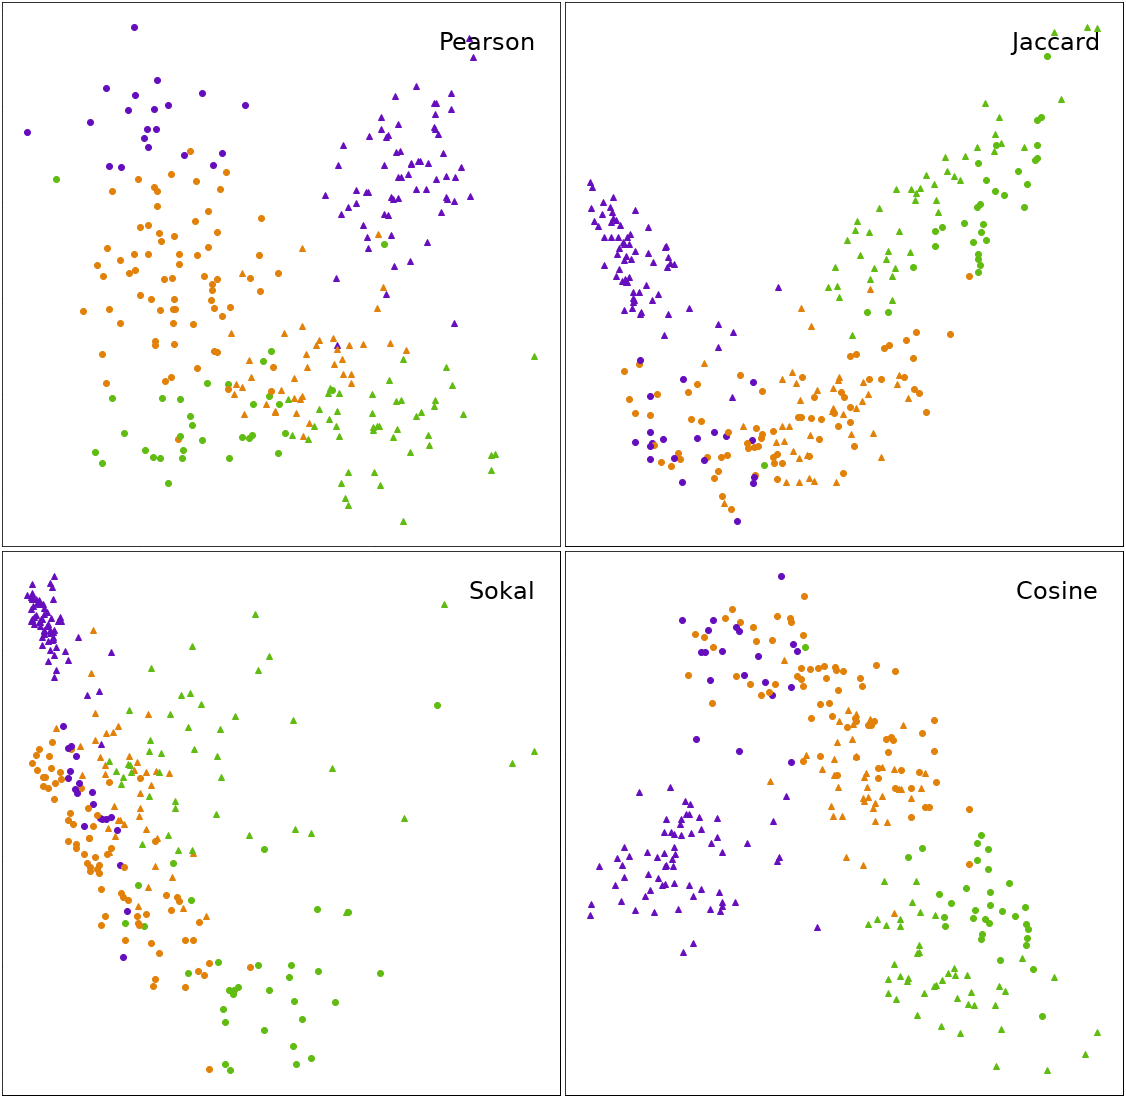
\includegraphics[height=8cm]{img/measures}
  \caption{Comparison of four similarity measures on same item-set}
  \label{fig:measures}
\end{figure}


% preserving of clusters

Figure \ref{fig:measures} shows four different similarity measures used on same data. Resulting projections are different. However, they all preserve information which is causing items from the same level and answer to form clusters. Different colors represent different levels and markers different answers.

% What different measurements measure

When we encounter performance matrix which contains only two (boolean) values, we can summarize the performance of all users on two items by using just four values using count of encountered answer pairs. See table \ref{tab:boolean-attributes}.

\begin{table}
  \begin{tabular}{ | l | l | l | }
      \hline
       & incorrect & correct \\ \hline
      incorrect & \ppl{$a$} & \ppl{$b$} \\ \hline
      correct & \ppl{$c$} & \ppl{$d$} \\ \hline
  \end{tabular}
  \caption{Four parameters of used boolean similarity measures}
  \label{tab:boolean-attributes}
\end{table}

\begin{itemize}
\item
  \textbf{Pearson} \ppl{$(ad - bc) / \sqrt{(a+b)(a+c)(b+d)(c+d)}$} \\ is commonly used. It correlates well with visibly simpler measure \textbf{Yule} ($(ad-bc)/(ad+bc)$).

\item
  \textbf{Jaccard} \ppl{$a / (a+b+c)$} differs visibly from other measures. Resulting projection still shows same clusters of levels and items are split based on a correct answer but similarity of the items does not correlate measures like Pearson. This is also mentioned later in evaluation chapter.

\item
  \textbf{Sokal} \ppl{$(a+d)/(a+b+c+d)$} shows best that different similarity measures can highlight different aspects of item performance. The similarity of items depends heavily on the performance of items when using Sokal. (Where performance of item is a number of correct answers divided by all answers.) Items with higher performance are much more similar than items with lower performance. This is causing a packed cluster of items from a first level (easy) and a spread out cluster of items from third level (harder).

\item
  \textbf{Cosine} \ppl{$a / \sqrt{ (a+b)(a+c) }$} similarity produces projection very similar to Jaccard.
\end{itemize}

So we can conclude that clusters are present despite used similarity measure.

% > Answers regularity

\section{Answers regularity}\label{evaulation-answers-regularity}

This section describes in detail some of our experiments we concluded which relates to separation of items into clusters of same correct answers. We describe four experiments in total which brought us from finding more properties of this regularity to determining cause in real dataset.

% > > Total similarity of items

\subsection{Total similarity of items}\label{total-similarity-of-items}

When exploring data, it may be useful to detect outliers. One possible way of how to detect an outlier is looking at sum of its similarities or distances to other $k$ nearest neighbors. This was done by [CITE]. In particular, this means that an item with a low sum of similarities to other items may be an outlier. This is where we encountered another regularity in data. It was detected that items with some correct answer may have greater similarity than other answers. This could cause problems with using such outlier detection as items having some correct answers have higher probability to be selected as outlier and its apparently not true.

Still, it is worth mentioning that this is not true for all similarity measures. It is apparent that Pearson and Cosine have this property but measures like Jaccard does not. It has different similarity for different levels instead. This is another difference between used similarity measures.

For this purpose we define another property of items - total similarity. It is a sum of one items vector of similarities to other items. (One column of similarity matrix). This property is normalized to range 0.0-1.0 and tells us how much is item similar to other items.

\begin{figure}
  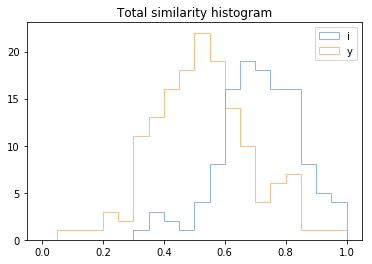
\includegraphics[width=10cm]{img/histogram_i_y}
  \caption{Histograms of total similarities of items divided by correct answer on one item-set}
  \label{fig:histogram_i_y}
\end{figure}

% total similarity histograms divided by answer

% other item-sets

This is not specific to only one item-set (which was used in previous images), almost all item-sets display similar pattern. Although for some item-sets, it's more distinct than for others. Sets consisting of items with many possible answers does not behave this way. But that is to be expected.

We picked few item-sets which have very distinct clusters of answers and looked whether the answer with higher similarity is located on left or on right in the user interface. Our finding was that there are item-set with a preferred answer on both left and right button. In particular in concept ``Vyjmenovaná slova'' which have possible answers ``i'' (left) and ``y'' (right) the preferred one is the left answer. But for concept ``Koncovky přídavných jmen'' which has the same possible answers is preferred one ``y'' on the right.

This experiment tells us only that there is some underlying difference between items with different correct answers but does not tell us what.

% > > Performance matrix

\subsection{Performance matrix}\label{performance-matrix}

After looking at performance matrix we can see that there are some rows which behavior differs greatly on different answers. This can be seen in figure \ref{fig:performance_matrix}. Each column in image depicts answers to one item. Each row corresponds to one user and colors represent correctness of answer (white is correct, black incorrect) or missing answer (red). Items are ordered in a way that all items having first of the answers as correct are on the left and items with another correct answer on the right.

\begin{figure}
  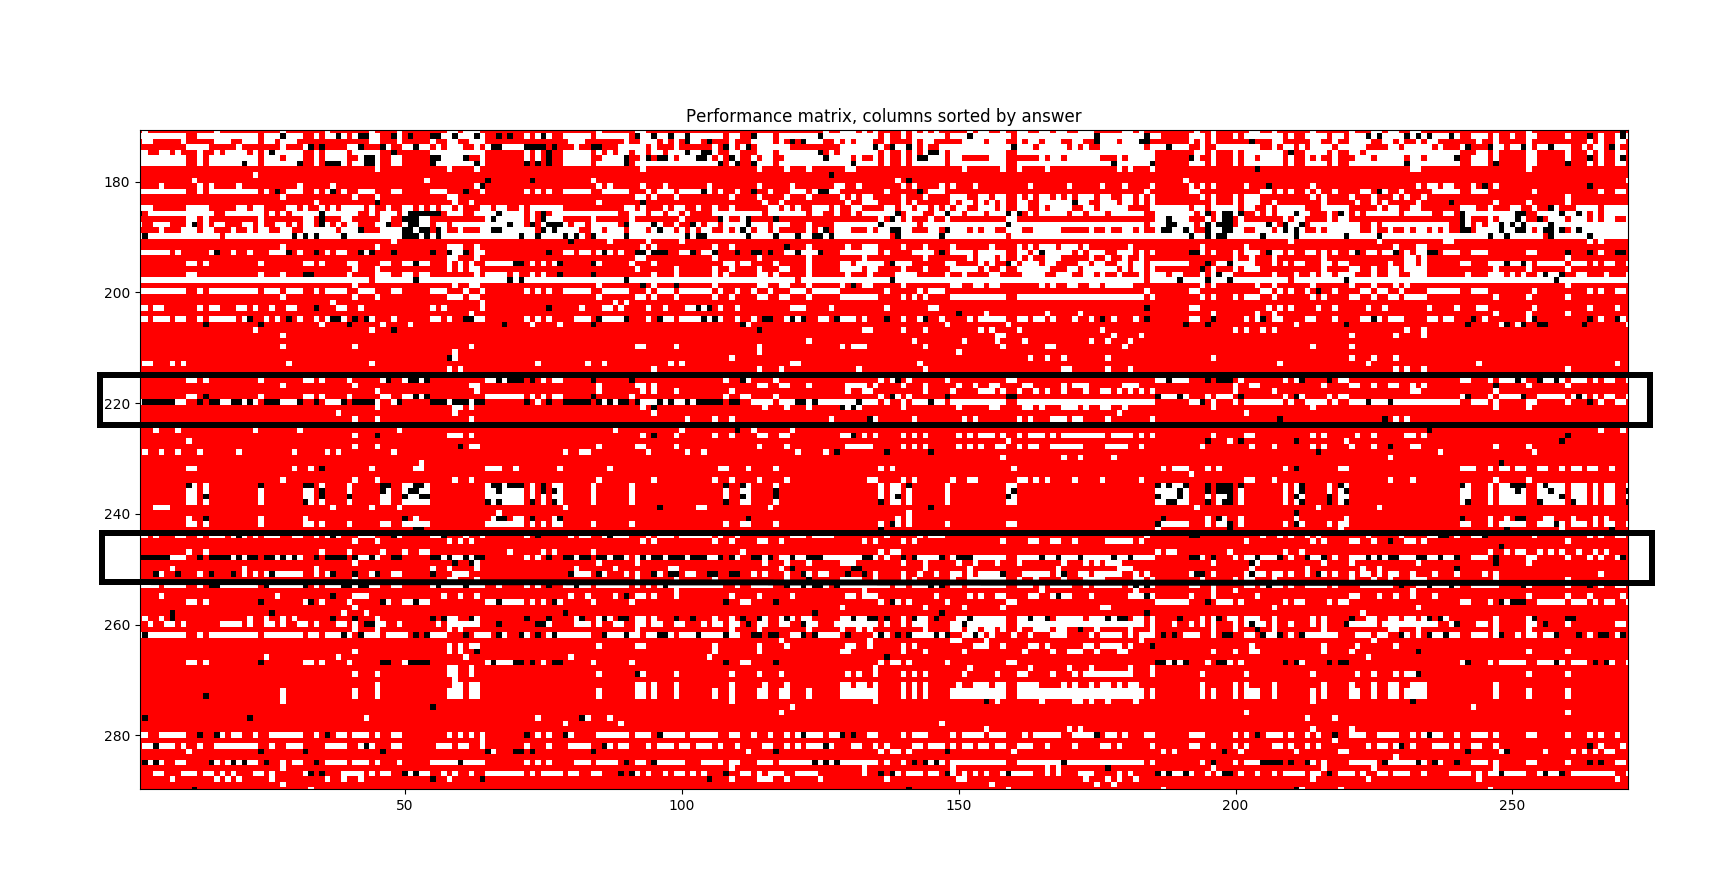
\includegraphics[width=10cm]{img/performance_matrix}
  \caption{Part of performance matrix with highlighted row contains uneven answers from single user}
  \label{fig:performance_matrix}
\end{figure}

After exploring performance matrix some more we can see that there are users who have much higher performance on items with one answer than another. There are even users who almost anyways use one of the answers. Such users are highlighted in the image. They answered almost all items with one answer (right) correctly and items with another answer (left) incorrectly.

% > > Default answer

\subsection{Default answer}\label{default-answer}

Our guess was that there are users who prefer using one answer by default when they do not know the answer. Firstly we wanted to determine whether preferring one answer over another can affect projection and create clusters of different answers.

We used simulation for this. Simulation is extended over basic simulation described in second chapter \ref{simulated-data}. There are a few differences over basic simulation. For each item, we also choose a correct answer. This is used to offset logistic function higher or lower to simulate higher chance of succeeding when solving items which correct answer is the users preferred one. In this experiment, we used offset 0.2 which corresponds to 20\% higher chance to answer correctly one answer and 20\% lower on items with another answer. Also, there are no missing values in performance matrix - simulated users answer to all items.

This specific simulation is using two uncorrelated skills and two answers. They are distributed in a way that there is the same amount of each combination (1/4 of items). We included different skills in this simulation to better illustrate conditions of real data - as such clusters of levels exist there.

\begin{figure}
  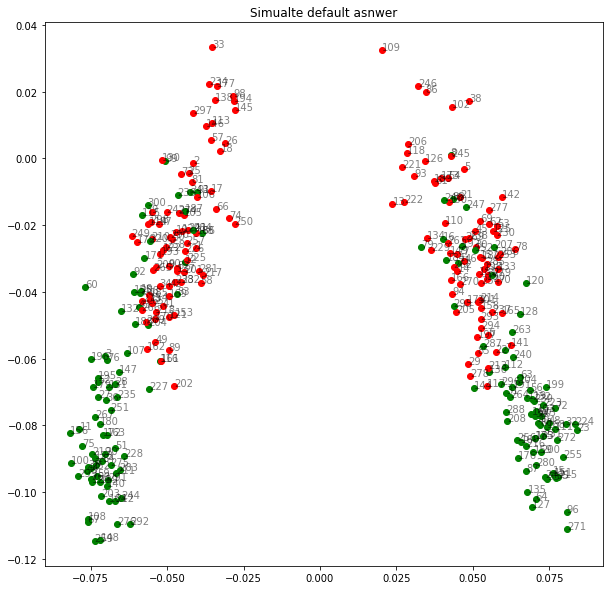
\includegraphics[height=8cm]{img/simulated_default}
  \caption{Projection of simulated data using default answers when user does not know how to answer}
  \label{fig:simulated_default}
\end{figure}

When we look at resulting projection \ref{fig:simulated_default} of simulated performance data we can see that it has same properties as our real data. There are clusters (in this case caused by uncorrelated skills) which have items separated by the correct answer (represented by different colors).

TODO better reasoning for this, explain why this happens

So users proffering one answer over another can cause items to separate by correct answer in projection.

% > > Filter out users

\subsection{Filter users}\label{filter-users}

% how to detect this in real data

The previous simulation showed that preferred answer can cause separation of items. Now we have to show that users like this exist in our real dataset.

We observed before that whole dataset uses both answers approximately the same, but for a single user this may not be true. In this experiment, we want to quantify whether each user prefers some answer or not. For this, we used a variation of user answer performances.

User answer performance is calculated as ratio of items which user answered correctly to all items when looking only at items with particular correct answer. We calculate this value for each possible correct answer and each user. Then we combine this set of user answer performances for each user to one value using their variance. This gives us single value representing whether user uses some answer by default. Value ranges from 0.0 which represents no preferred answer at all to 0.5 which is largest possible preference.

\begin{figure}
  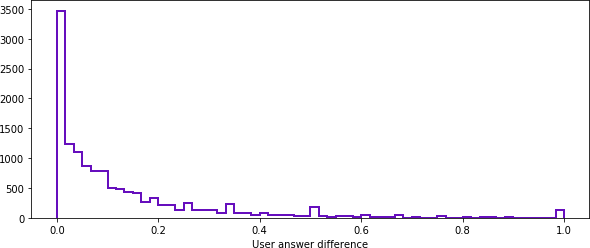
\includegraphics[width=10cm]{img/uneven_answers_hist}
  \caption{Histogram of user answer performance difference}
  \label{fig:uneven_answers_hist}
\end{figure}

Figure \ref{fig:uneven_answers_hist} shows histogram of this values calculated for each user on one item-set. There are few visible groups of users. The largest group have uniform performance on all answers (represented by values close to 0.0). On the other end of the spectrum are users who use only one answer (values close to 1.0). And in the middle, there are users who probably prefer one answer but use both answers. It is visible, that there is quite a large amount of users with a small preference for one of the answers. (It does not matter which one.)

% similar items from different levels are little closer to each other

We can use this to filter out users which difference in performance is too large. We thought that this will remove the separation of items based on a correct answer from a projection. And it does. Figure \ref{fig:answers_normalization} shows projection before and after filtering users based on their answer performance difference. In this particular case, we consider that user should be filtered out when his difference on answers is greater than 0.06 which is median value. Colors in this particular image represent correct answers of items.

\begin{figure}
  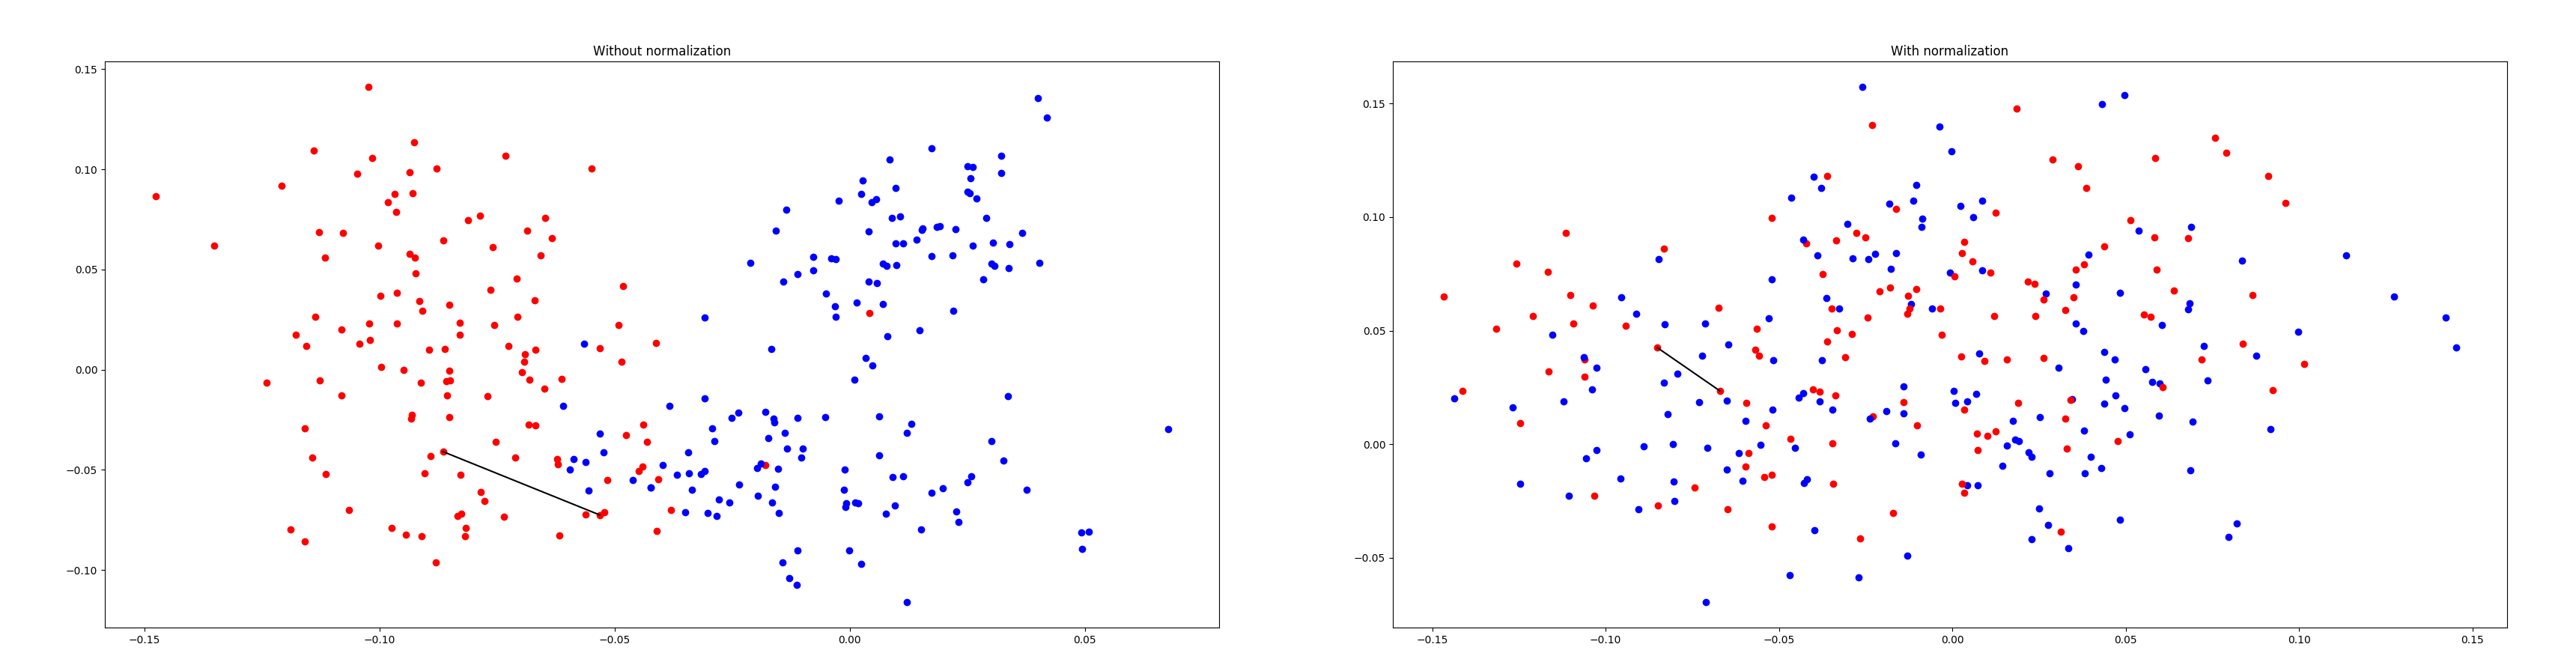
\includegraphics[width=\textwidth]{img/answers_normalization}
  \caption{Effect of filtering out users}
  \label{fig:answers_normalization}
\end{figure}

In section \ref{regularities-level-regularity} of the second chapter we also mentioned that there are words in different levels which should be appear closer to each other than they do using simple pipeline. Such pair of words is shown in figure \ref{fig:answers_normalization} with the black straight line connecting them. Distance between them shrank. But this also caused that that all possible answers are now mixed together. One could argue whether this is better or worse than before as questions with different answers in our particular tutoring system probably should not be as similar. But this depends on goal of use-case for which is similarity used.

% is these too many users removed?

When we use only half of users which performance is more uniform separation of items with same answers is gone. Its half of users because we compare their difference to median difference. Apparent question is whether a smaller amount of users removed may not be enough. Transition between both extremes is continuous - on one end is total separation of items with different answers and on the another they are totally mixed. There is no visible jump between this states.

We look at the performance of items instead of how much user uses each answer because we do not have to normalize it in any way. If we choose to use usage of answers we have to compare this to correct ratio as it is not guaranteed that item-set contains same amount of items for all correct answers. Using variance of performance resolves this for us automatically.

% answer regularity short summary

To sum it up. When we simulated users we gave them all habit to use one answer more commonly. This divided items by their corresponding correct answer. But not all users have a habit of using one answer by default in real-world data. Yet there is quite a large amount of users who do. We can filter them out to stop them affecting projections.

% > Levels regularity

\section{Levels regularity}\label{evaulation-levels-regularity}

This section describes in detail some of our experiments we concluded which relates to formation of items into clusters of same level. The section contains two experiments sowing some factors which can affect similarity in such manner that clusters forms.

% > > Missing values

\subsection{Missing values}\label{missing-values}

% Can missing data affect result of similarity calculation?

As we mentioned before, performance matrix is relatively sparse. Though missing values are not distributed randomly - they form a distinct pattern. Our question is whether this pattern of missing values can affect similarity of items and projections.

% structure of performance matrix

Items in each item-set of the system are divided into up to three levels. As the difficulty of levels is differs users in the system usually do not solve all of the available levels. Less experienced users tend to solve only first or first two levels. Still, more experienced users solve only higher levels. This is causing visible pattern in performance matrix. Some user rows contain information only about specific levels and are missing all values of other levels.

Based on this we can divide users into 8 groups. All groups are listen in table \ref{tab:user-groups}. First three columns say whether this group contains users who solved particular levels. We say that user solved level when he answered at least 30 items (which is 1/3 of questions for observed item-set). We added color to each group so we can distinguish them in following plots easily. Groups are not represented in data uniformly. Most of the users fall into two groups. These two groups are users who either solve only first or only second level.

\begin{table}
  \begin{tabular}{ | l | l | l | l | l | }
    \hline
      1   & 2   & 3   & Color      & Users \\ \hline
      no  & no  & no  & black      & 35\%  \\ \hline
      yes & no  & no  & red        & 31\%  \\ \hline
      no  & yes & no  & green      & 9\%   \\ \hline
      no  & no  & yes & blue       & 8\%   \\ \hline
      yes & yes & no  & yellow     & 7\%   \\ \hline
      no  & yes & yes & cyan       & 2\%   \\ \hline
      yes & no  & yes & magenta    & 2\%   \\ \hline
      yes & yes & yes & light gray & 7\%   \\ \hline
  \end{tabular}
  \caption{Groups of users}
  \label{tab:user-groups}
\end{table}

% simulation of missing values

Once again, we used simulated data to gather more information about this. A simulation was concluded in the same way as we explained before in section \ref{simulated-data}. The only difference is that resulting performance matrix will now contain missing values. We wanted to recreate missing data in a similar way that this occurs in real performance matrix. This is achieved by simulated users not solving all items. Each user starts with solving one level and then with some probability continues to another. So most users solve only one level, some users solve 2 levels and only a few users solve all 3 levels. Order in which they answer levels is chosen at random as users are not required to continue chronologically. This is also visible in real data - there are users who solve only second or only highest difficulty level.

% What can one answer possibly affect in different matrices (value in performance matrix, row and column in similarity and all in projection or second level of similarity)

\begin{figure}
  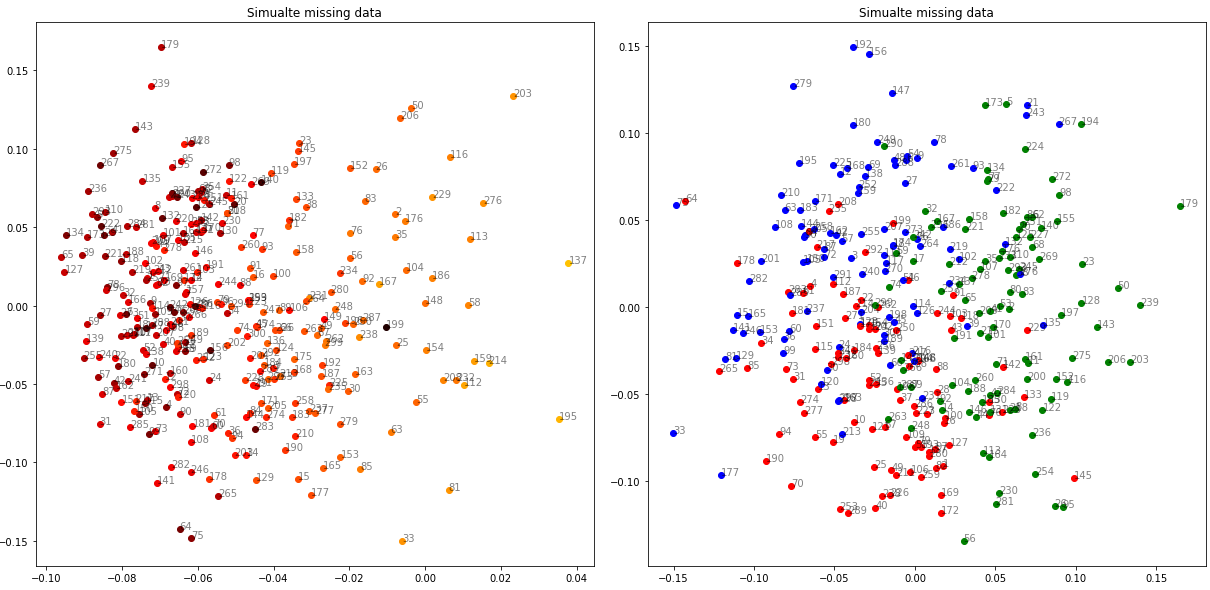
\includegraphics[width=\textwidth]{img/simulated_missing}
  \caption{First and second (left) and second and third (right) principal components of PCA on simulated data; image on left is colored by difficulty of items}
  \label{fig:simulated_missing}
\end{figure}

Figure \ref{fig:simulated_missing} shows projection of our simulated data with missing answers. Projection on left shows first two principal components of PCA, projection on right shows second and third component of PCA. So there are 3 dimensions shown effectively. Colors in the first image depict difficulty of items (dark are difficult, light simple items). The second image is colored by levels as usual.

In this case first dimension corresponds pretty well with difficulty of items and next two dimensions (second image) distinguish belongingness to each level. Such easy explanation of axis is possible only for simulated data. When looking at projections of real data it is much harder to say anything about its axis.

After looking at similarity matrix we saw that there is difference between similarities in same level and similarities of items in different levels. For given amount of items, mean levels solved by single user and number of users there is visible difference in stability of similarity results. Computed similarities for items in same level are much more stable than in between levels. This may cause specific used use-case (in this case projection) to consider items in same level as more similar.

Yet this is not true true in general only if amount of users who solved items in more than one level is small. If we increase number of simulated users by 10 times we will get stable similarity and no clusters.

% > > Item performance

\subsection{Item performance}\label{item-performance}

As we know items are divided into in such manner that difficulty of levels raises. Question is whether this is directly projected into similarity of items.

\begin{figure}
  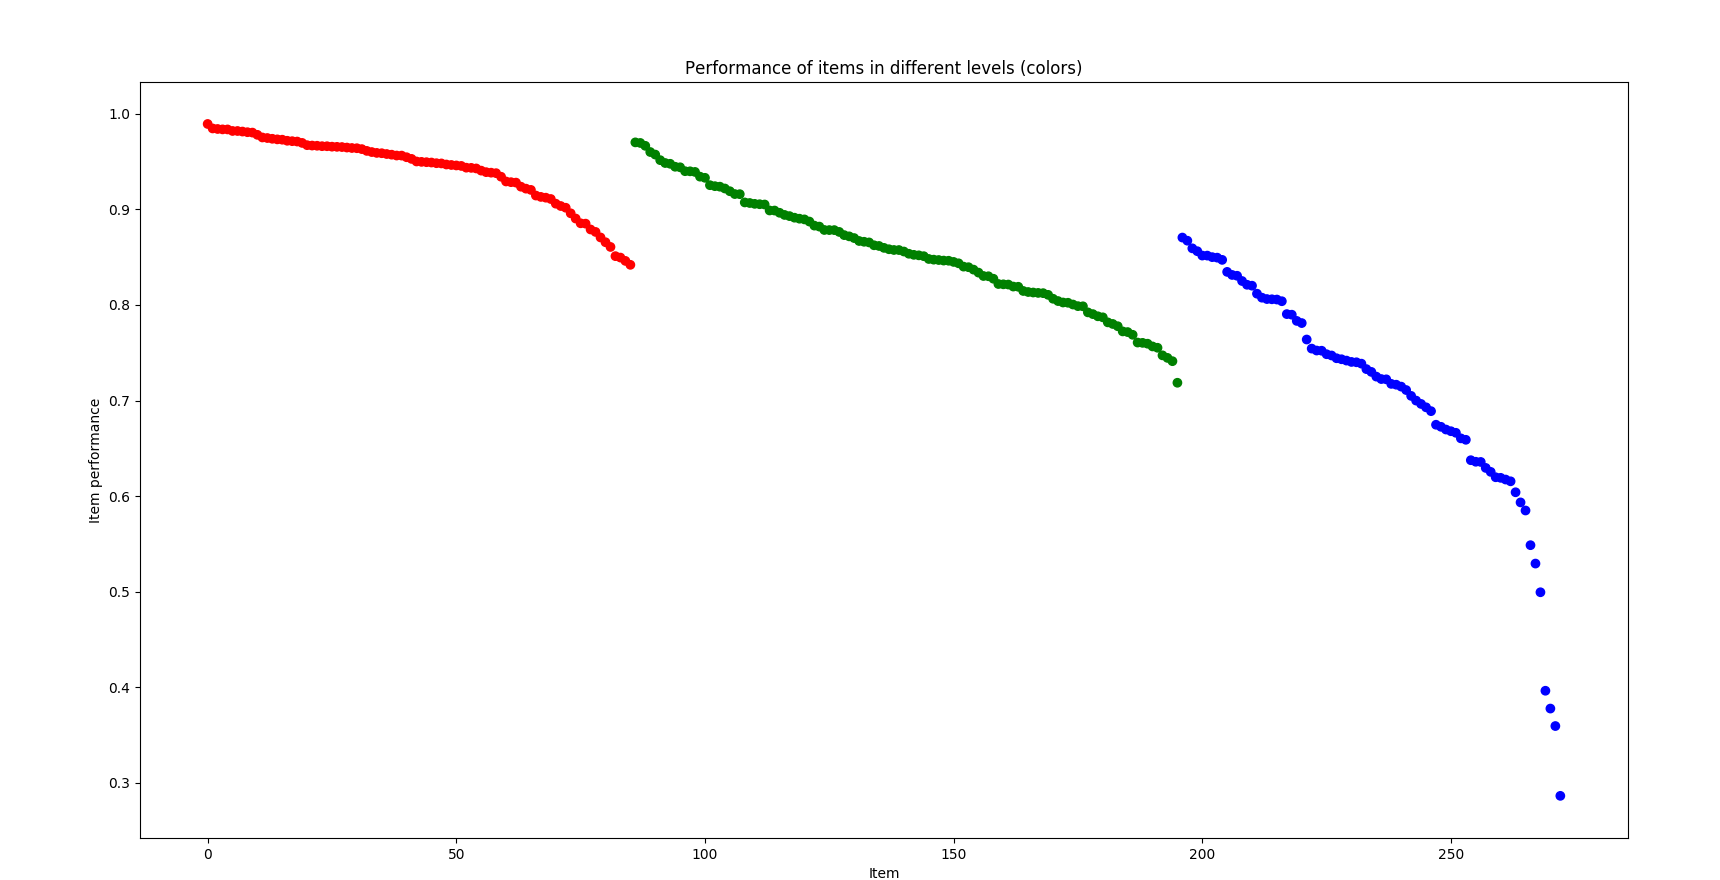
\includegraphics[width=10cm]{img/items_performance_levels}
  \caption{Mean performance of items in three levels of single item-set}
  \label{fig:item_performance_levels}
\end{figure}

Figure \ref{fig:item_performance_levels} shows mean items performance (ratio of correct answers to all answers) from one item-set. Horizontal axis contains items sorted by level and mean their performance. The vertical axis shows a performance of each item. Given item-set contains three item-sets with mean performance 94\%, 86\%, 71\% respectively.

TODO more text about this

% different performance of items in levels does not cause such clusters

%

% > Notebook

\section{Notebook}\label{notebook}

Concluded experiments are collected in Jupyter Notebooks which also use scripts written in python to simplify our work and make notebooks cleaner. There are also some additional experiment not described in this text. Providing all the experiments in this way gives everyone possibility to alter and re-execute them. More information about launching this environment is present in enclosed files.

\chapter{Recommendations}\label{recommendations}

% --------------------------- %
% Recommendations             %
% --------------------------- %

% superintro

This short chapter summarizes recommendations gathered after looking at results of our experiments.

% intro, affected portion of data on different stages of pipeline

As we have learned there are a few stages used in our pipeline for computing similarity. We come from raw logs through calculated similarity to some its use-case. Diagram \ref{fig:affected_diagram} depicts possible effect of single value changed in log of users performance. Apparently, in performance matrix, this is only single value. When we continue with computing similarity matrix single row and single column can be affected in some way. On this level it is still straightforward - answers to item affect similarities which include this item. Although, when we apply some additional level of processing like clustering, dimensionality reduction, or second level of similarity each changed value can affect all of the items. At this we compare each item to each item.

\begin{figure}
  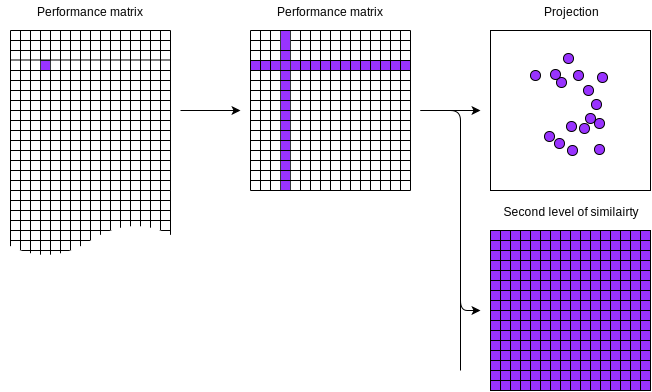
\includegraphics[width=10cm]{img/affected_diagram}
  \caption{Diagram of possibly affected values on different stages of processing}
  \label{fig:affected_diagram}
\end{figure}

Yet, as we know, single changed value does not change much. It is underlying truth about items and users that affect similarity measures. This also shows that chosen pipeline is robust and complex as it allows us to uncover hidden information in performance data.

This work consists mostly of exploitative analysis of similarity measures and their use cases on dataset from \umimeCesky{}. Especialy we focused on using data about user performance from single exercise. At the beginning we knew about existence of some regularities in data that caused clusters of items that were same in some way that should not be present in the used data. On a way for explaining them we found multiple high-level factors that can possibly affect results of calculated similarity and projections of items in tutoring systems. We also encountered some problems and therefore can give some recommendations for future work in this or comparable area.

% > General recommendations

\section{General recommendations}\label{general-recommendations}

As we saw, when using similarity with some specific dataset problems specific for it may arise. While trying to explain this patterns in our particular used data we run into multiple situations which can repeat even when explaining some different data using similarity techniques.

% determine range

I think it is always good idea to first determining range of effect. E. g., whether this problem also appears when we use some different measure or data. I know it is basic. But it can be easily forgotten when facing some specific problem. And it was in great help to us. Such experiments were explained in first section \ref{evaluation-basic} of previous chapter.

% simulations

I found it useful to use simulations when we are dealing with techniques from which we obtain some results but it is hard to explain why (projection). Altering inputs and observing output is a way for explaining what is happening inside.

% more dimensions of PCA

Usually when using PCA only first two principal components are used but I found it useful to look at more some other dimensions as well. This approach was used in section \ref{missing-values} when first dimension correlated with difficulty of items and did not give us any useful information.

\section{Practical recommendations}\label{practical-recommendations}

TODO this text

% in visualizations

This work did not focus on differnet possible visualisations of items, but as byproduct of concluded experiments we still made some.

projection
simples one
for each item-set seaprately


% in outlier detection

For outlier detection we can recommend

using method that does not depend on global dsitribution of values, only on local neighborhood
or
use same normalization, for example proposed removal of users with great preference for one answer causing this separation of items. But other less drastic normalization method can also be found we only used this one to show that this is a cause for this clusters.

% in ...

% Limitations
\section{Limitations}\label{limitations}

There were some limitations forced by source of data we used, and some decisions were made for simplicity or other explained reasons. For our analysis we used only one exercise type - simple ``fill-in-the-blank'' with choice from two answers. Also only information about performance was used for computing similarity of items, other sources of data were ignored as we thought that this source of data may bring most unexpected results. But there may arise other problems when using different sources of data. And performance was used only as correctness of answer - we did not include time it took users to solve item into consideration. This is probably correct path to take in studied tutoring system but it may be important to also incorporate solving time into performance in some other systems.

\chapter{Conclusion}

% --------------------------- %
% Conclusion                  %
% --------------------------- %

% What we did, what important discoveries we found,..

We explored differences in using different methods for measuring similarity of educational items based on data about correctness of users answers. Prior to starting this work we knew there were some unclear circumstances considering formation of clusters in projection and therefore distribution of similarities of items. All the experiments we concluded were focused on this behavior. Now we understand how structure of system may affect performance data and similarity of items itself.

We determined whether is this unclear behavior present in all data and as part of this we also compared different similarity measures. Multiple experiments using simulated data were concluded. And as the result we are pretty sure about cause of one of the regularities and proposed some high-level factors that can cause other observed regularity. As in real data there may be multiple factors causing any information in the data it is not straightforward to explain clusters of items from same level.

Most of the findings discovered on this dataset may not be directly transferable to other tutoring system. But used analysis can also help understand other tutoring systems. Or maybe even systems which are not used for learning but contains items with similar properties.

% Ideas for future work,..

This work was concluded as exploration analysis and hence its results consists mostly of gathered information and recommendations for future work. In particular implementing proposed recommendations when using similarity of items in mentioned tutoring system. Similarity of items is currently not used in the system \umimeCesky{} but increasing number of items will soon call for some automated management of problem pool. For this reason it will be useful to further analyze methods for detecting problems with item pool.

In particular compare usefulness of different methods of item visualizations for human judgment. Also implementation of automatic detection of duplicate and outlier items may be useful. In some special cases it may be even possible to recommend kinds of items that are missing from the system using similarity of items.

% Recapitulation of how well we finished our task,..

After concluding all this I think given task was fulfilled. TODO

% See ya

\makeatletter\thesis@blocks@clear\makeatother
%\phantomsection %% Print the index and insert it into the
%\addcontentsline{toc}{chapter}{\indexname} %% table of contents.
%\printindex

\appendix %% Start the appendices.
\chapter{An appendix}

\begin{table}
  \begin{tabular}{ | l | l | l | l | }
    \hline
       & min & median & max \\ \hline
      delka-samohlasek-i & 0.272173 & 0.572914 & 0.733154 \\ \hline
      delka-samohlasek-u & 0.179007 & 0.218907 & 0.278768 \\ \hline
      koncovky-mi-my-ma & 0.173923 & 0.378383 & 0.574999 \\ \hline
      koncovky-ovi-ovy & -0.022328 & 1.000000 & 1.000000 \\ \hline
      koncovky-podstatnych-jmen-muzsky-rod & 0.460326 & 0.526986 & 0.652672 \\ \hline
      koncovky-podstatnych-jmen-stredni-rod & 0.444935 & 0.859304 & 0.880381 \\ \hline
      koncovky-podstatnych-jmen-zensky-rod & 0.358566 & 0.423671 & 0.501532 \\ \hline
      koncovky-pridavnych-jmen & 0.431434 & 0.500458 & 0.558587 \\ \hline
      me-mne-samostatne-zajmeno-ja & -0.012182 & 0.289142 & 1.000000 \\ \hline
      predlozky-s-z & 0.31752 & 0.413021 & 0.455101 \\ \hline
      psani-be-bje & -0.009319 & 0.671716 & 1.000000 \\ \hline
      psani-me-mne-ve-slove & 0.646219 & 0.733133 & 0.733133 \\ \hline
      psani-nn-a-n & 0.305013 & 0.409739 & 0.462562 \\ \hline
      psani-s-c-s-z & 0.288553 & 0.353498 & 0.44766 \\ \hline
      psani-ve-vje & -0.013296 & 1.000000 & 1.000000 \\ \hline
      shoda-podmetu-s-prisudkem & 0.189355 & 0.245732 & 0.306245 \\ \hline
      sklonovani-zajmen-jez-jenz-nimz-ji & -0.01751 & 0.121347 & 0.353978 \\ \hline
      slovesa-podminovaci-zvratna & 0.06066 & 0.10416 & 0.173317 \\ \hline
      tvrde-a-mekke-souhlasky & 0.135091 & 0.257167 & 0.832182 \\ \hline
      vyjmenovana-slova-po-b & 0.385475 & 0.597867 & 0.637596 \\ \hline
      vyjmenovana-slova-po-l & 0.575217 & 0.641585 & 0.837544 \\ \hline
      vyjmenovana-slova-po-m & 0.478953 & 0.928013 & 0.943975 \\ \hline
      vyjmenovana-slova-po-p & 0.641131 & 0.832391 & 0.88884 \\ \hline
      vyjmenovana-slova-po-s & 0.373571 & 0.421781 & 0.446662 \\ \hline
      vyjmenovana-slova-po-v & 0.483608 & 0.678045 & 0.722796 \\ \hline
      vyjmenovana-slova-po-z & 0.528562 & 0.565708 & 0.657444 \\ \hline
  \end{tabular}
  \caption{Quality of clusters in different item-sets}
  \label{tab:quality-of-clusters}
\end{table}

\end{document}
